\documentclass[%
  a4paper,    
  parskip=half,
  twoside=true,
  %openright,      % start new chapters on an even-numbered page (right)
  draft=false,
]{scrreprt}

% **************************************** 
% Information
% **************************************** 
\newcommand{\thesisTitle}{Generierung angepasster RDF-Dumps von Wikidata}
\newcommand{\thesisName}{Benno Fünfstück}
\newcommand{\thesisSubject}{Bachelorarbeit}
\newcommand{\thesisDate}{Oktober 15, 2019}
\newcommand{\thesisVersion}{My First Draft}

\newcommand{\thesisFirstReviewer}{Prof. Dr. Markus Krötzsch}
\newcommand{\thesisFirstReviewerUniversity}{\protect{Technische Universität Dresden}}
\newcommand{\thesisFirstReviewerDepartment}{Fakultät Informatik}

\newcommand{\thesisSecondReviewer}{Prof. Sebastian Rudolph}
\newcommand{\thesisSecondReviewerUniversity}{\protect{Technische Universität Dresden}}
\newcommand{\thesisSecondReviewerDepartment}{\protect{Fakultät Informatik}}

\newcommand{\thesisFirstSupervisor}{Prof. Markus Krötzsch}
\newcommand{\thesisSecondSupervisor}{Prof. Sebastian Rudolph}

\newcommand{\thesisUniversity}{\protect{Technische Universität Dresden}}
\newcommand{\thesisUniversityDepartment}{Fakultät Informatik}
\newcommand{\thesisUniversityInstitute}{Institut für Theoretische Informatik}
\newcommand{\thesisUniversityGroup}{Professur für Wissensbasierte Systeme}
\newcommand{\thesisUniversityCity}{}
\newcommand{\thesisUniversityStreetAddress}{01062 Dresden}
\newcommand{\thesisUniversityPostalCode}{}

% **************************************** 
% Load and Configure packages 
% **************************************** 

% setup german for XeLaTeX
\usepackage{polyglossia}
\setmainlanguage[spelling=new,babelshorthands=true]{german}
\usepackage{fontspec}

\PassOptionsToPackage{% setup clean thesis style
  figuresep=colon,%
  hangfigurecaption=false,%
  hangsection=true,%
  hangsubsection=true,%
  sansserif=false,%
  configurelistings=true,%
  colorize=full,%
  colortheme=bluemagenta,%
  configurebiblatex=true,%
  bibsys=biber,%
  bibfile=bib-refs,%
  bibstyle=alphabetic,%
  bibsorting=nty,%
}{cleanthesis}
\usepackage{cleanthesis}

\hypersetup{% setup the hyperref-package options
  pdftitle={\thesisTitle},    %   - title (PDF meta)
  pdfsubject={\thesisSubject},%   - subject (PDF meta)
  pdfauthor={\thesisName},    %   - author (PDF meta)
  plainpages=false,           %   -
  colorlinks=false,           %   - colorize links?
  pdfborder={0 0 0},          %   -
  breaklinks=true,            %   - allow line break inside links
  bookmarksnumbered=true,     %
  bookmarksopen=true          %
}

\usepackage{cleveref}
\usepackage{bookmark}
\usepackage{changepage}
\usepackage{xsavebox}

% avoid large space before paragraphs with title
\RedeclareSectionCommand[beforeskip=0pt]{paragraph}

\newcommand{\introterm}[1]{\emph{#1}}

\usepackage{tikz}
\usetikzlibrary{shapes.geometric}
\usetikzlibrary{calc}

\newenvironment{tikzcomponent}[1]{%
  \begin{xlrbox}{#1}%
    \begin{tikzpicture}%
    }{
    \end{tikzpicture}%
  \end{xlrbox}%
}


\begin{document}

\frenchspacing

\pagenumbering{roman}			% roman page numbing (invisible for empty page style)
\pagestyle{empty}				% no header or footers
% !TEX root = ../my-thesis.tex
%
% ------------------------------------  --> cover title page
\begin{titlepage}
	\pdfbookmark[0]{Cover}{Cover}
	\flushright
	\hfill
	\vfill
	{\LARGE\thesisTitle \par}
	\rule[5pt]{\textwidth}{.4pt} \par
	{\Large\thesisName}
	\vfill
	\textit{\large\thesisDate} \\
	Version: \thesisVersion
\end{titlepage}


% ------------------------------------  --> main title page
\begin{titlepage}
	\pdfbookmark[0]{Titlepage}{Titlepage}
	\tgherosfont
	\centering

	{\Large \thesisUniversity} \\[6mm]
	\textsf{\thesisUniversityDepartment} \\
	\textsf{\thesisUniversityInstitute} \\
	\textsf{\thesisUniversityGroup} \\

	\vfill
	{\large \thesisSubject} \\[5mm]
	{\LARGE \color{ctcolortitle}\textbf{\thesisTitle} \\[10mm]}
	{\Large \thesisName} \\

	\vfill
	\begin{minipage}[t]{.27\textwidth}
		\raggedleft
		\textit{1. Gutachter}
	\end{minipage}
	\hspace*{15pt}
	\begin{minipage}[t]{.65\textwidth}
		{\Large \thesisFirstReviewer} \\
	  	{\small \thesisFirstReviewerDepartment} \\[-1mm]
		{\small \thesisFirstReviewerUniversity}
	\end{minipage} \\[5mm]
	\begin{minipage}[t]{.27\textwidth}
		\raggedleft
		\textit{2. Gutachter}
	\end{minipage}
	\hspace*{15pt}
	\begin{minipage}[t]{.65\textwidth}
		{\Large \thesisSecondReviewer} \\
	  	{\small \thesisSecondReviewerDepartment} \\[-1mm]
		{\small \thesisSecondReviewerUniversity}
	\end{minipage} \\[10mm]
	\begin{minipage}[t]{.27\textwidth}
		\raggedleft
		\textit{Betreuer}
	\end{minipage}
	\hspace*{15pt}
	\begin{minipage}[t]{.65\textwidth}
		\thesisFirstSupervisor
	\end{minipage} \\[10mm]

	\thesisDate \\

\end{titlepage}


% ------------------------------------  --> lower title back for single page layout
\hfill
\vfill
{
	\small
	\textbf{\thesisName} \\
	\textit{\thesisTitle} \\
	\thesisSubject, \thesisDate \\
	Reviewers: \thesisFirstReviewer\ and \thesisSecondReviewer \\
	Supervisors: \thesisFirstSupervisor\ and \thesisSecondSupervisor \\[1.5em]
	\textbf{\thesisUniversity} \\
	\textit{\thesisUniversityGroup} \\
	\thesisUniversityInstitute \\
	\thesisUniversityDepartment \\
	\thesisUniversityStreetAddress
}
		% INCLUDE: all titlepages
\cleardoublepage

\pagestyle{plain}				% display just page numbers
% !TEX root = ../my-thesis.tex
%
\pdfbookmark[0]{Abstract}{Abstract}
\addchap*{Abstract}
\label{sec:abstract}

\blindtext

\vspace*{20mm}

{\usekomafont{chapter}Abstract (different language)}
\label{sec:abstract-diff}

\blindtext
		% INCLUDE: the abstracts (english and german)
\cleardoublepage
%
%% !TEX root = ../my-thesis.tex
%
\pdfbookmark[0]{Acknowledgement}{Acknowledgement}
\addchap*{Acknowledgement}
\label{sec:acknowledgement}

\Blindtext[2][2]
 % INCLUDE: acknowledgement
%\cleardoublepage
%
\currentpdfbookmark{\contentsname}{toc}
\setcounter{tocdepth}{2}		% define depth of toc
\tableofcontents				% display table of contents
\cleardoublepage

% --------------------------
% Body matter
% --------------------------
\pagenumbering{arabic}			% arabic page numbering
\setcounter{page}{1}			% set page counter
\pagestyle{scrheadings}			% header and footer style

\typeout{CONTENT START NOW}
% !TEX root = ../thesis.tex
%
\chapter{Einleitung}
\label{sec:intro}
Wikipedia ist die bekannteste freie Wissenssammlung im Internet.
Bei fast 50 Millionen Artikeln in 278 Sprachen\footnote{\url{https://stats.wikimedia.org/DE/TablesArticlesTotal.htm} (alle URLs in dieser Arbeit wurden am 01.10.2019 abgerufen)} Anfang 2019 sind Informationen zu einer Vielfalt an Themen verfügbar.
Sogar YouTube und Facebook greifen auf Wikipedia zurück, um zusätzliche Informationen zu kontroversen Themen zu präsentieren \cite{youtube-facebook-wp}.

Die Darstellung der Informationen in natürlicher Sprache als Textartikel ist für Menschen praktisch.
Die Extraktion von Fakten für die maschinelle Verarbeitung aus diesen Textartikel ist jedoch schwierig \cite{oie-errors,extract-rel-ibm}.
Das Problem wird durch die unterschiedlichen Sprachversionen noch verstärkt, denn die beschriebenen Fakten können sich je nach Sprache unterscheiden.
Als Lösung wurde 2012 das Wikidata Projekt gegründet, mit dem Ziel, die Informationen aus Wikipedia in atomare Aussagen zerlegt strukturiert zu verwalten \cite{wikidata}.

Die Daten aus Wikidata sind für viele Anwendungen aufgrund von zwei Merkmalen besonders interessant.
Erstens ist Wikidata wie Wikipedia ein Community-Projekt.
Die Daten stehen unter einer freien Lizenz und können von jedem ergänzt und korrigiert werden.
Deswegen enthält Wikidata Informationen zu einer Vielzahl an Themengebieten.
Zweitens besitzt Wikidata ein vielfältiges Datenmodell.
Je nach Art der Bestimmung kann beispielsweise entweder der Mount Everest oder Chimborazo als höchster Punkt der Erde gesehen werden.
Wikidata kann beide Sichtweisen abbilden, wie \cref{fig:sample-statement} zeigt.
Um die Herkunft einer Information zu belegen, kann jeder Fakt mit Referenzen versehen werden.

Aus der Größe von Wikidata ergeben sich Herausforderungen.
Im September 2019 hat die Größe des vollständigen Exports der Daten als GZip\footnote{\url{http://www.gzip.org/}}-komprimiertes JSON\footnote{JavaScript Object Notation (\url{https://www.json.org})} 60 GB überschritten.\footnote{\url{https://web.archive.org/web/20190930113616/https://dumps.wikimedia.org/wikidatawiki/entities/}}
Für viele Anwendungen sind aber nicht alle Daten relevant.
Ziel dieser Arbeit ist deswegen die Entwicklung eines Systems zum einfachen Abruf einer Teilmenge dieser Daten.

\begin{figure}
  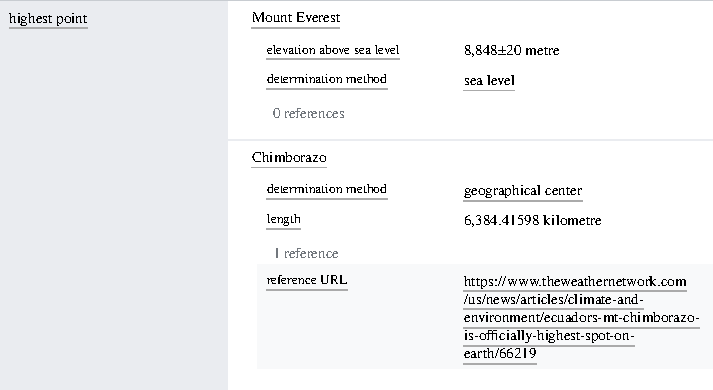
\includegraphics[width=\linewidth]{pics/example-statement}
  \caption{Zwei Statements des Items "`Erde"' für die Property "`höchster Punkt"'}
  \label{fig:sample-statement}
\end{figure} 

Eine bereits existierende Möglichkeit zur Abfrage von Daten ist der Wikidata Query Service \cite{wd-sparql}. 
Mit diesem Service lassen sich komplexe Abfragen auf den Daten von Wikidata beantworten.
Da die Laufzeit von Abfragen auf eine Minute limitiert ist, eignet sich dieser allerdings nicht für große Datenmengen.
Das dieses Limit nicht nur ein theoretisches Problem ist, zeigt eine Arbeit zur Verwendung von Referenzen in Wikidata\cite{wd-wk-common-references}.
Die Autoren mussten die Abfrage nach allen Referenzen von einem Mitarbeiter von Wikimedia Deutschland ausführen lassen, da sie nicht innherhalb des Limits terminiert.
Ein weiteres Problem ist die sehr feine Zerlegung der Daten beim Wikidata Query Service.
Während damit der Zugriff auf spezifische Informationen einfach ist, wird es schwierig, alle Informationen zu einem Thema abzurufen.

Das in dieser Arbeit vorgestellte System füllt die Nische zwischen dem vollständigen Export und dem Wikidata Query Service.
Durch die Angabe von Filtern wird eine Teilmenge der Daten definiert.
Aus den Daten, die diese Filter erfüllen, wird dann ein individualisierter Datenexport (Dump) generiert.
Über eine Integration mit dem Archivierungsdienst Zenodo\footnote{\url{https://zenodo.org/}} können die generierten Dumps direkt archiviert werden.
Zenodo generiert einen Digital Object Identifier (DOI), sodass die Dumps danach einfach in wissenschaftlichen Veröffentlichungen zitiert werden können.

\section{Struktur der Arbeit}
Im zweiten Kapitel wird zunächst notwendiges Hintergrundwissen zum Aufbau von Wikidata und den verwendeten Technologien vermittelt.
Danach werden in \cref{chap:requirements} die Anforderung an das System detaillierter beschrieben und verwandte Arbeiten verglichen.
In \cref{chap:design} wird dann das Design des Systems erarbeitet, dessen Implementierung in \cref{chap:implementation} vorgestellt wird.
Die Evaluation der Implementierung auf Korrektheit und Vollständigkeit erfolgt in \cref{chap:evaluation}, mit einem  Vergleich zwischen den existierenden Wikidata-Dumps und den generierten Dumps.
Im \cref{chap:conclusion} wird schließlich ein Ausblick auf mögliche Verbesserungen gegeben und eine Zusammenfassung des Ergebnis präsentiert.

Dabei werden die folgenden Beiträge geleistet:
\begin{itemize}
  \item Analyse verschiedener Systemdesigns zur Generierung angepasster Wikidata-Dumps
  \item Entwurf einer Spezifikation für Filterkriterien
  \item Implementierung des vorgestellten Designs mit Wikidata Toolkit\footnote{https://github.com/Wikidata/Wikidata-Toolkit}. Wikidata-Toolkit ist eine Bibliothek zum Verarbeiten und Erzeugen von Wikidata Dumps.
  \item Evaluation der Vollständigkeit und Korrektheit des RDF-Exports von Wikidata Toolkit
\end{itemize}  
% !TEX root = ../thesis.tex
%
\chapter{Hintergrund}
\label{sec:concepts}
In diesem diesem Kapitel werden Grundlagen zu Wikidata und RDF\footnote{\url{https://www.w3.org/RDF/}} (Resource Description Framework), einem Standardformat zur Beschreibung von Informationen, erklärt. 

\section{Wikidata als strukturiertes Wiki}
Wikidata ist die gemeinsame Wissensdatenbank der Wikimedia Projekte.
Wie auch Wikipedia selbst baut Wikidata auf MediaWiki\footnote{\url{https://mediawiki.org}} auf, einer Software für das Betreiben von kollaborativen Wikis.
Im Gegensatz zu Wikipedia verwaltet Wikidata jedoch strukturierte Dokumente.
Die Erweiterungen für MediaWiki dazu stellt das Wikibase\footnote{\url{htts://wikiba.se}} Projekt bereit.

Alle Dokumente in Wikidata besitzen einen eindeutigen Identifier.
Dieser beginnt mit einem Großbuchstaben, der den Typ des Dokuments angibt, gefolgt von einer Zahl.
Aktuell kennt Wikidata drei Typen von Dokumenten: Items (Q), Properties (P) und Lexemes (L).
Lexemes wurden erst später hinzugefügt, so dass sie von dem in dieser Arbeit verwendeten Wikidata-Toolkit noch nicht vollständig unterstützt werden.
In dieser Arbeit werden Lexemes daher nicht genauer betrachtet.

Den Hauptbestandteil der Daten bilden jedoch die Items.
Ein Item repräsentiert ein bestimmtes Konzept, zu dem Fakten in Wikidata erfasst werden.
Der Aufbau eines Items ist beispielhaft anhand von \verb|Q42| (Douglas Adams) in \cref{fig:wd-datamodel} dargestellt.
Den ersten Teil bilden die Terme: \verb|label|, \verb|description| und \verb|aliases| dienen zur Beschreibung und Definition des Items.
Die Terme sind mehrsprachig: ein Item kann ein \verb|label| für jede der möglichen Sprachen haben.
Darauf folgen Statements, welche die Fakten zu diesem Item wiedergeben.
Zusätzlich kann jeder Item noch eine Reihe an Sitelinks besitzen. 
Diese verlinken auf andere Seiten des Wikimedia Projekts zum Thema des Items.
Die Sitelinks von \verb|Q42| verlinken zum Beispiel auf Artikel von Douglas Adams in den unterschiedlichen Sprachversionen von Wikipedia und in Wikiquote.

Die Fakten eines Items werden in Statements beschrieben.
Ein Statement besteht aus zwei Teilen: einem Claim, der eine bestimmte Aussage trifft, und einer Liste von Referenzen.
Da auch Statements ohne Referenzen erlaubt sind, kann die Liste der Referenzen auch leer sein.
Wikidata unterstützt drei Arten von Aussagen, genannt Snaks:
\begin{description}
\item[PropertyValue] die am meisten verwendete Art einer Aussage. Sie beschreibt den Fakt, dass eine bestimmte Eigenschaft (Property) einen gewissen Wert (Value) hat. Die Property bestimmt dabei den Typ der Value. Values können je nach Property andere Items oder skalare Werte (wie Zahlen, Zeichenketten, Koordinaten, Zeiten, usw.) sein.
\item[SomeValue] diese Art der Aussage wird verwendet, um auszudrücken, dass ein Wert für die Eigenschaft existiert der aber nicht bekannt ist. Zum Beispiel kann die Aussage ``es existiert ein Wert für den Todeszeitpunkt einer Person'' verwendet werden, falls eine Person gestorben ist, der Todeszeitpunkt aber nicht bekannt ist.
\item[NoValue] drückt aus, dass es für eine bestimmte Eigenschaft keinen Wert gibt. Wird verwendet, wenn das Fehlen einer Information keine Unvollständigkeit darstellt. Kann zum Beispiel für \verb|P200| (Zuflüsse) verwendet werden, wenn ein Gewässer keine Zuflüsse besitzt. 
\end{description}
Der Claim eines Statements besteht aus einem MainSnak, der die Hauptaussage darstellt, und zusätzlichen Qualifiern zur Verfeinerung der Aussage.
Eine Referenz ist auch einfach eine Liste von Snaks. 
Ein MainSnak zu Douglas Adams (Q42) ist zum Beispiel \verb|P69| (educated at) - \verb|Q691283| (St John's College).
Mit den Qualifier-Snaks wie \verb|P582| (end time) - \verb|1974| bildet dieser dann einen Claim.
Das Statement setzt sich dann aus diesem Claim und der Liste von Referenzen zusammen.
Alle Statements für die gleiche Property werden in einer Statement Group zusammengefasst.
Jedes Statement besitzt zusätzlich noch einen Rank (deprecrated, normal oder best) um die Priorität innerhalb der Statement Group auszudrücken.

Dieses Dokument-orientierte Datenmodell lässt sich einfach als JSON\footnote{\url{https://www.json.org}} (JavaScript Object Notation) repräsentieren.
Die vollständige Darstellung ist jedoch sehr umfangreich und ist deshalb aus Platzgründen hier nicht abgebildet.
Für ein Entity kann die JSON-Repräsentation einfach online abgerufen werden, für \verb|Q42| zum Beispiel unter folgender URL: \url{https://www.wikidata.org/wiki/Special:EntityData/Q42.json}.
Zusätzlich stellt Wikidata Exporte aller Dokumente als JSON bereit.

\begin{figure}
  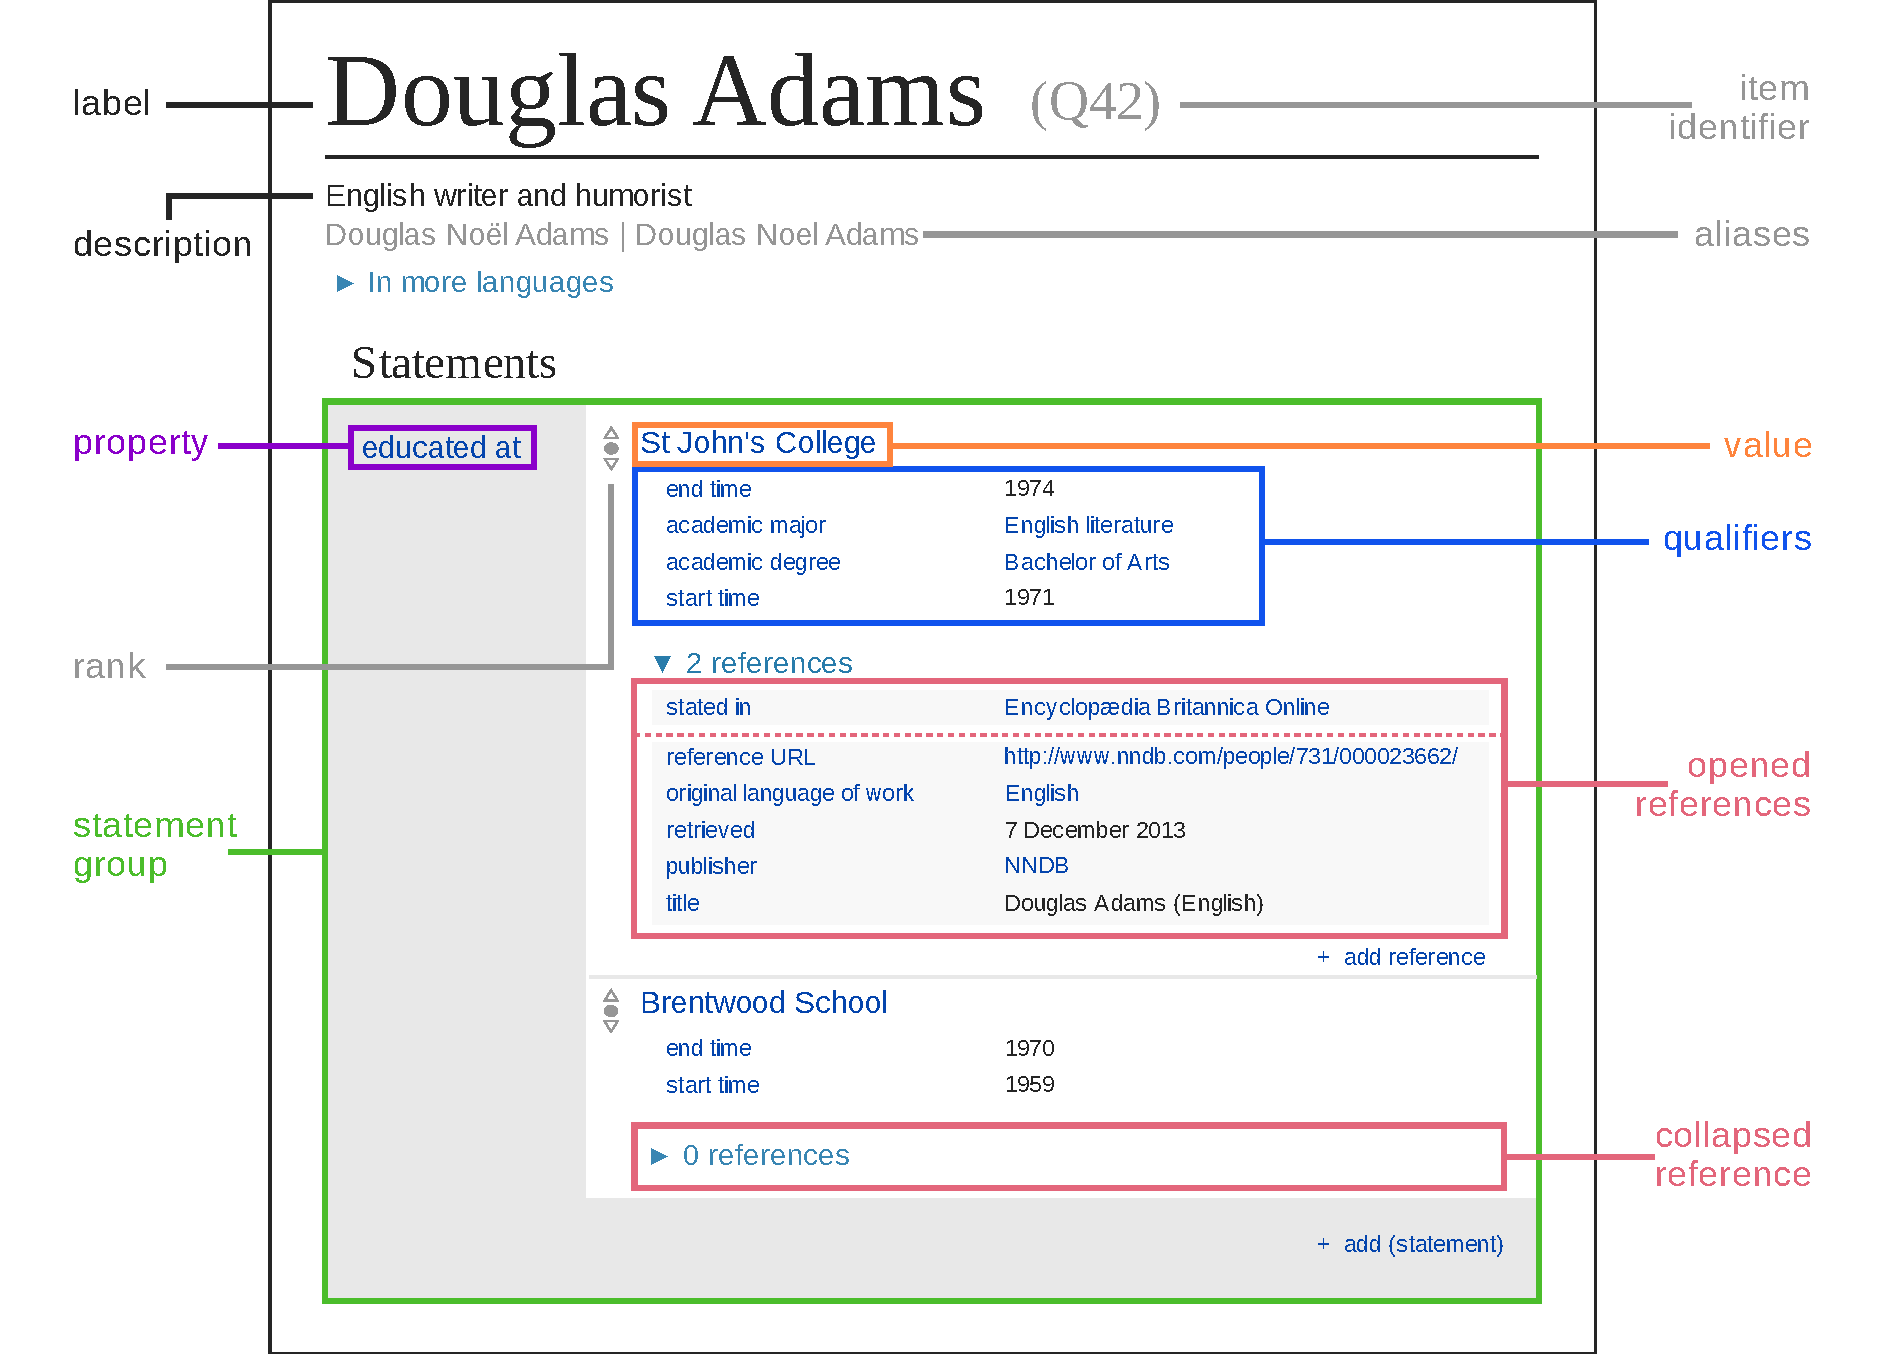
\includegraphics[width=\linewidth]{pics/Datamodel_in_Wikidata}
  \caption{Wikidata Item ``Q42''}
  \label{fig:wd-datamodel}
\end{figure}

\section{Wikidata als Linked Data}
Eine Besonderheit von Wikidata ist die starke Verlinkung der Daten untereinander.
Diese Verlinkung ermöglicht eine Art des Zugriffs, die sich von der dokumentbasierten Betrachtungsweise unterscheidet.
Fragestellungen wie ``Wer sind die Verwandten von Douglas Adams?'' oder ``Welche berühmten Personen sind in einem Staat geboren, der Mitglied der europäischen Union ist?'' betrachten die Beziehungen der Dokumente, und nicht allein den Inhalt einzelner Dokumente.

Das W3C hat für solche Graph-basierten Daten das Resource Description Framework (RDF) entwickelt.
In RDF werden als eindeutige Bezeichner Internationalized Resource Identifiers (IRIs)\footnote{https://www.ietf.org/rfc/rfc3987.txt} verwendet.
IRIs sind eine Erweiterung von URIs zur Unterstützung von internationalen Zeichensätzen.
In der Praxis werden für IRIs oft HTTP URLs verwendet, sodass Namenskonflikte zwischen unterschiedlichen Organisationen vermieden werden.
Außerdem können über HTTP weitere Informationen zu der entsprechenden Ressource bereitgestellt werden.

Das Kernelement von RDF bilden Tripel. Die drei Komponenten jedes Tripel sind:
\begin{description}
\item[Subjekt] eine IRI oder Blank Node
\item[Prädikat] eine IRI
\item[Objekt] eine IRI, Blank Node oder Literal
\end{description}
Blank Nodes sind lokale Bezeichner, die im Gegensatz zu IRIs nur innerhalb eines Dokuments eindeutig sein müssen.
Verschiedene RDF Dokumente können daher die selben Blank Node Bezeichner verwenden, ohne dass damit die selbe Resource beschrieben wird.

Literale in RDF sind Zeichenketten, die jedoch zusätzlich noch einen Datentypen oder einen Language Tag besitzen können.
Mit dem Datentyp kann die Interpretation der Zeichenkette genauer spezifiziert werden.
Auch Datentypen werden über IRIs referenziert.
Language Tags geben die Sprache der Zeichenkette als Language Code nach BCP47\footnote{\url{https://tools.ietf.org/html/bcp47}} an. In diesem Fall muss der Datentyp \url{http://www.w3.org/1999/02/22-rdf-syntax-ns#langString} sein.

RDF Dokumente sind eine Kollektion von Tripeln, wobei die Reihenfolge keine Rolle spielt.
Für die Serialisierung von RDF gibt es verschiedene Standards, ein einfacher und verbreiteter ist N-Triples\footnote{\url{https://www.w3.org/TR/n-triples/}}.
Die Syntax von N-Triples ist in folgendem Beispiel examplarisch dargestellt:
\begin{lstlisting}[language=SPARQL, breaklines=true]
<https://example.org> <http://schema.org/name> "Beispiel"@de .
<https://example.org> <http://schema.org/name> "Example"@en .
_:paper <https://example.org/about> <https://example.org> .
_:paper <https://example.org/popularity> "42"^^<http://www.w3.org/2001/XMLSchema#integer> .
\end{lstlisting}
Jede Zeile entspricht einem Tripel und wird mit einem Punkt abgeschlossen.
In N-Triples werden IRIs in \verb|<>| eingeschlossen und Blank Nodes durch das Prefix \verb|_:| markiert.
Literale sind von \verb|"| umgeben, mit \verb|@| bzw \verb|^^| können Language Tag und Datentyp angegeben werden.

In dieser Arbeit wird zur Übersichtlichkeit eine Erweiterung der Notation verwendet.
Dabei werden IRIs durch die Einführung von den in \cref{tab:rdf-prefixes} aufgeführten Prefixen vereinfacht.
Zum Beispiel wird \verb|<http://schema.org/name>| als \verb|schema:name| abgekürzt. 

\begin{table}
\begin{tabular}{l l}
\bfseries{Prefix} & \bfseries{URL} \\
rdf: & <http://www.w3.org/1999/02/22-rdf-syntax-ns\#> \\
xsd: & <http://www.w3.org/2001/XMLSchema\#> \\
% ontolex: & <http://www.w3.org/ns/lemon/ontolex\#> \\
% dct: & <http://purl.org/dc/terms/> \\
rdfs: & <http://www.w3.org/2000/01/rdf-schema\#> \\
owl: & <http://www.w3.org/2002/07/owl\#> \\
skos: & <http://www.w3.org/2004/02/skos/core\#> \\
schema: & <http://schema.org/> \\
% cc: & <http://creativecommons.org/ns\#> \\
geo: & <http://www.opengis.net/ont/geosparql\#> \\
prov: & <http://www.w3.org/ns/prov\#> \\
wikibase: & <http://wikiba.se/ontology\#> \\
wdata: & <http://www.wikidata.org/wiki/Special:EntityData/> \\
% bd: & <http://www.bigdata.com/rdf\#> \\
wd: & <http://www.wikidata.org/entity/> \\
wdt: & <http://www.wikidata.org/prop/direct/> \\
wdtn: & <http://www.wikidata.org/prop/direct-normalized/> \\
wds: & <http://www.wikidata.org/entity/statement/> \\
p: & <http://www.wikidata.org/prop/> \\
wdref: & <http://www.wikidata.org/reference/> \\
wdv: & <http://www.wikidata.org/value/> \\
ps: & <http://www.wikidata.org/prop/statement/> \\
psv: & <http://www.wikidata.org/prop/statement/value/> \\
psn: & <http://www.wikidata.org/prop/statement/value-normalized/> \\
pq: & <http://www.wikidata.org/prop/qualifier/> \\
pqv: & <http://www.wikidata.org/prop/qualifier/value/> \\
pqn: & <http://www.wikidata.org/prop/qualifier/value-normalized/> \\
pr: & <http://www.wikidata.org/prop/reference/> \\
prv: & <http://www.wikidata.org/prop/reference/value/> \\
prn: & <http://www.wikidata.org/prop/reference/value-normalized/> \\
wdno: & <http://www.wikidata.org/prop/novalue/>
\end{tabular}
\caption{Verwendete Prefixe. Diese werden auch vom Wikidata SPARQL Service vordefiniert.}
\end{table}

RDF kennt weder Referenzen noch Qualifier und kann im Gegensatz zu Wikidata auch nicht mehrere gleiche Tripel speichern.
Erxleben, Günther, Krötzsch, Mendez und Vrandečić haben 2014 beschrieben, wie trotzdem eine Darstellung als RDF möglich ist und auch ein System zur Erstellung regelmäßiger Exporte als RDF entwickelt \cite{wikidata-rdf-export}.
Nach dem Prinzip der Reifikation werden Statements, Referenzen und komplexe Werte nicht direkt als Tripel exportiert, sondern als eigene Ressourcen. 
Diese Ressourcen besitzen dann ein Tripel das zu dem Objekt des Statements verlinkt, aber auch zusätzlich Tripel für Qualifier und Referenzen.
Jedes Statement hat somit einen eindeutigen Namen, sodass auch zwei Statements mit dem selben Inhalt erfasst werden können.
\begin{figure}
  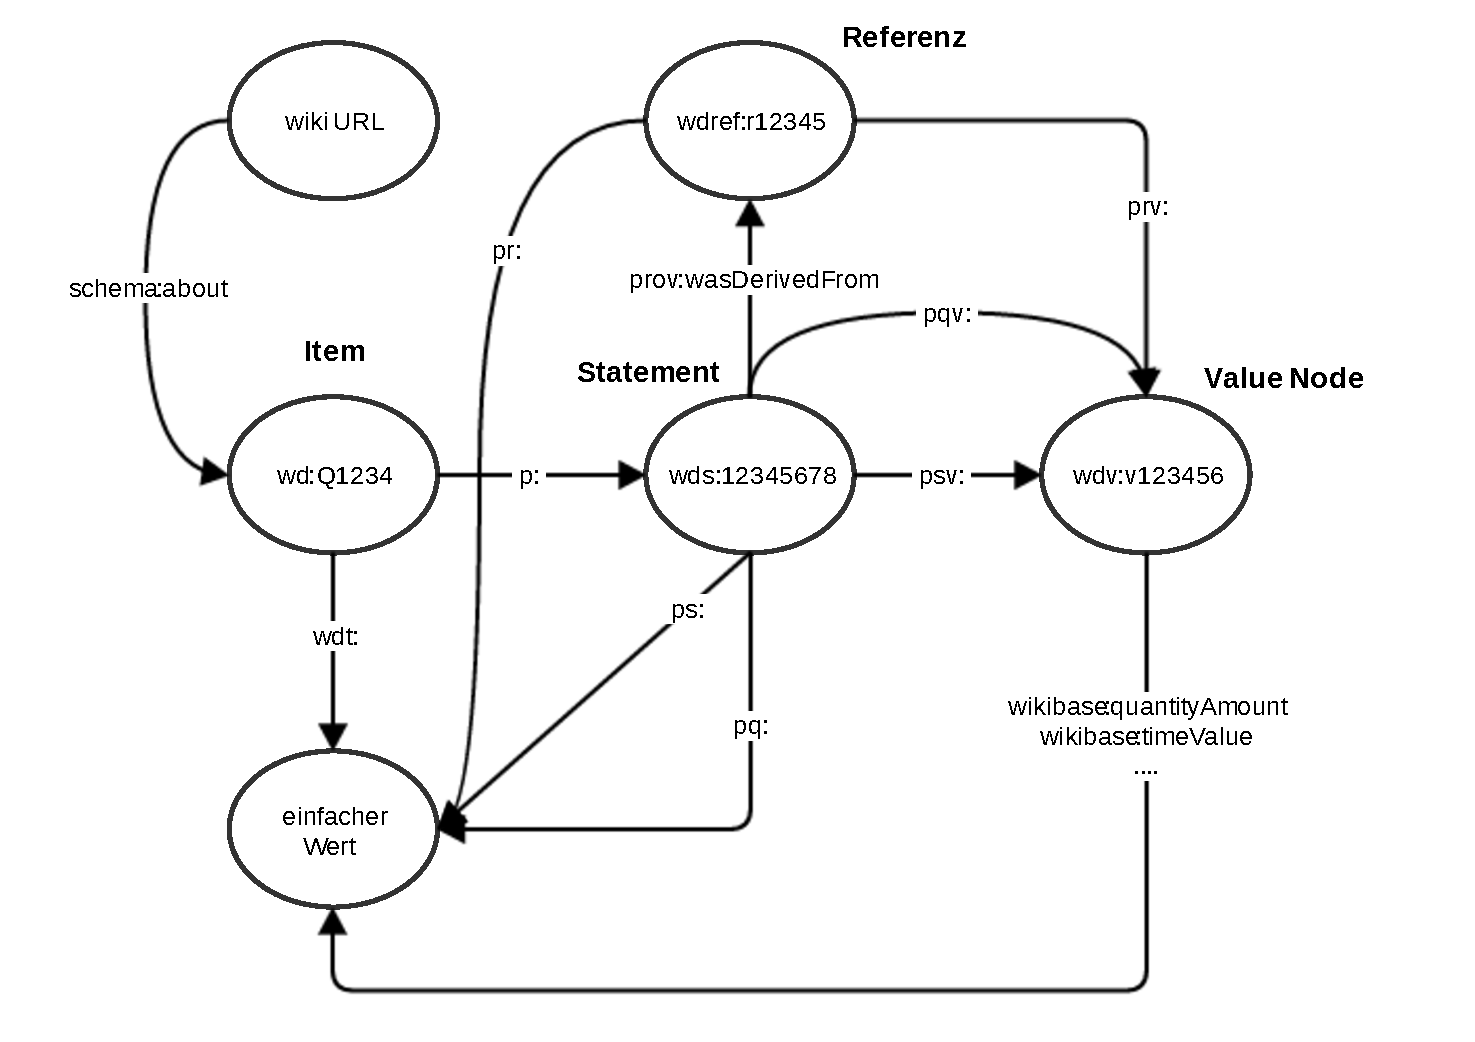
\includegraphics[width=\linewidth]{pics/Rdf_mapping}
  \caption{Mapping des Datenmodells auf RDF}
  \label{fig:rdf-mapping}
\end{figure}

Diese Übersetzung ist in \cref{fig:rdf-mapping} gezeigt.
Jeder Pfeil beschreibt dabei Prädikatprefix, welches dann für RDF-Tripel verwendet wird.
An dieses Präfix wird der Bezeichner der Property angehangen.
Hier ist ein Beispiel zur Verdeutlichung (gekürzt, die Informationen zu den Reference und Value Nodes sind nicht abgebildet):
\begin{lstlisting}[language=SPARQL]
wd:Q42 p:P26 wds:q42-xxxx .
wds:q42-xxxx rdf:type wikibase:Statement .
wds:q42-xxxx ps:P26 wd:Q14623681 .
wds:q42-xxxx pq:P580 "1991-11-25T00:00:00Z"^^xds:dateTime .
wds:q42-xxxx pqv:P580 wdv:c8ae0d38443d4671d3f893d7000a859e .
wds:q42-xxxx pq:P582 "2001-05-11T00:00:00Z"^^xsd:dateTime .
wds:q42-xxxx pqv:P582 wdv:1c30ade7914d072877b2db404a683d7c .
wds:q42-xxxx prov:wasDerivedFrom wdref:yyyyyyyy .
wd:Q42 wdt:P26 wd:Q14623681 .
\end{lstlisting}
Das Beispiel zeigt, wie die Property \verb|P26| (spouse) zuerst mit dem Prädikat \verb|p:P26| auf das Statement verlinkt.
Das Statement verlinkt dann über \verb|ps:P26| zum einfachen Wert der Property.
Mit \verb|pq:P580| (start time) bzw. \verb|pqv:P580| wird auf die einfache und komplexe Darstellung des Wertes für diesen Qualifier verlinkt.
Die komplexe Darstellung enthält noch weitere Informationen zu dem Datum, wie bspw. die Genauigkeit oder das verwendete Kalendermodell.

Eine spezielle Bedeutung hat der \verb|wdt:| Prefix.
Tripel mit diesen Prädikaten verlinken Items direkt mit den einfachen Werten.
Diese Tripel existieren allerding nur dann, wenn das zugehörige Statement vom Typ \verb|BestRank| hat.
Dieser Typ umfasst alle Statements, die den höchsten Rang für diese Property haben und nicht deprecrated sind.
Solche Statements und Tripel werden auch als ``truthy'' bezeichnet.
Die truthy Tripel sind sehr hilfreich, wenn man nicht an Qualifiern, Referenzen oder komplexeren Werten interessiert ist.
Für diesen Fall bieten sie eine einfachere Sicht auf die Daten, was besonders bei Abfragen die Komplexität reduziert.
      
\chapter{Anforderungen}

\section{funktionale Anforderungen}
Im Fokus dieser Arbeit steht die Entwicklung eines Systems zur Filterung des RDF-Exports von Wikidata.
Damit sollen Wissenschaftler mit wenig Aufwand Dumps nach speziellen Kriterien erstellen können.
Die wesentlichen Merkmale des Systems sind:

\begin{description}
  \item[Format] Der Dump soll als RDF im N-Triples Format erstellt werden. Damit die gefilterten Dumps möglichst kompatibel mit dem vollständigen Wikidata RDF Dump sind, sollte das Schema dem offiziellen RDF-Dump-Format entsprechen. Erweiterungen des Schemas müssen klar gekennzeichnet sein.
  \item[Filterung] Nutzer sollen über eine einfache Oberfläche wählen können, welche Entitäten in welchem Detailgrad im erstellten Dump enthalten sind. 
  \item[Archivierung] Damit die Dumps in wissenschaftlichen Veröffentlichungen zitiert werden können, muss die Verfügbarkeit auch in ferner Zukunft garantiert werden. Deshalb ist eine Methode zur Langzeitarchivierung generierter Dumps notwendig. 
  \item[Suche] es soll eine durchsuchbare Übersicht über alle erstellen Dumps.
    So können Ideen anderer Nutzer als Vorlage dienen und nicht jeder Nutzer muss sich eigene Filterregeln ausdenken,
  \item[Statistiken] Um schnell zu entscheiden, ob ein Dump für einen bestimmten Anwendungsfall geeignet ist, sollten Statistiken über den Inhalt (z.B. die Anzahl der Entitäten) des Dumps angezeigt werden. Zusätzlich sollten auch schon während der Generierung Statistiken zum Fortschritt des Dumps bereitgestellt werden.
  \item[Nachvollziehbarkeit] Gerade für den wissenschaftlichen Einsatz ist es erforderlich, dass die Herkunft der Daten und Generierung nachvollziehbar ist. Es sollte demnach leicht sichtbar sein, wie der Dump entstanden ist und eine Reproduktion des Dumps mit diesen Daten möglich sein. 
  \item[Aktualität der Daten] Die Dumps sollten aus möglichst aktuellen Daten erstellt werden.
    Es ist natürlich nicht notwendig, dass die Dumps immer komplett aktuell sind, aber die Daten zur Generierung der Dumps sollten regelmäßig aktualisiert werden.
\end{description}

\section{nicht-funktionale Anforderungen}
Neben den Anforderungen an die Funktion des Systems existieren auch eine Reihe von weiteren Anforderungen:

\begin{description}
  \item[Hardwareanforderungen] Der Ressourcenverbrauch des Systems sollte in einem akzeptablen Rahmen liegen.
  Als Anhaltspunkte für die Beurteilung dienen hier vergleichbare Systeme, wie bspw. der Wikidata Query Service, welcher ebenfalls Services basierend auf den RDF-Daten von Wikidata anbietet und gleichzeitig deutlich populärer ist. Demnach sollte das System entsprechend seiner Relevanz geringere Hardwareanforderungen als der Wikidata Query Service haben.
\item[Freie Lizenz] Die Wikimedia Foundation legt großen Wert darauf, möglichst viele der verwendeten Tools unter einer freien Lizenz bereitzustellen\cite{wikimedia-guiding-principles}.
  Wenn das System in der Wikimedia Cloud betrieben werden soll, dann ist die Veröffentlichung des Quellcodes unter einer freien Lizenz sogar Pflicht\cite{wikimedia-cloud-tos}.
\item[Bearbeitungszeit] Das System sollte maximal einen Tag zur Generierung eines Dumps benötigen, besser unter 12 Stunden. Während längerer Prozesse sollte keine ständig Verfügbarkeit des Nutzers erwartet werden. 
\item[Erweiterbarkeit] Da die funktionalen Anforderungen an das System sehr allgemein sind, muss auf Erweiterbarkeit geachtet werden sodass neue Anforderungen einfach umgesetzt werden können. Es sind beispielsweise viele verschiedene Filtermöglichkeiten und Statistiken denkbar, die nicht alle in der ersten Version umgesetzt werden können. Es ist daher sinnvoll vor allem in diesem Bereich auf Erweiterbarkeit zu achten.
\item[Skalierbarkeit] Wikidata wächst beständig, aktuell existieren etwas weniger als 59 Millionen Items.\TODO{cite}
  Insgesamt gibt es über 700 Millionen Statements und diese Zahl ist allein im letzten Jahr um 200 Millionen gewachsen. Das System muss also mit dieser Menge an Daten umgehen können und dies auch für die nächsten Jahre noch leisten können.
\end{description}

\section{Verwandte Arbeiten}
 
SPARQL query service
Linked Data Fragments
Dbpedia Topical Dumps
Wikidata REST API
Wikidata Toolkit
petscan/catscan  
\chapter{Design}
\label{chap:design}
In diesem Kapitel werden die Anforderungen präzisiert und ein Design für die Umsetzung erarbeitet.
Dazu sind mehrere Aspekte relevant: zum einen die technische Umsetzung der Filterung und Generierung von Dumps (Architektur und unterstützte Filterkriterien), zum anderen die Gestaltung des User-Interfaces und die Auswahl externen Dienste (z.B. für die Archivierung der erzeugten Dumps).
Diese bedingen sich gegenseitig: es ist wenig sinnvoll, wenn die Architektur sehr komplexe Filterkriterien unterstützt, dass User-Interface das aber gar nicht abbilden kann (oder umgekehrt).

\section{Architektur}
Für die Architektur der Anwendung stellt sich zuerst die Frage, wie die Arbeit zwischen Server und Client verteilt werden soll.
Auf der einen Seite steht die Variante, einen schlauen Client zu entwickeln, welcher direkt mit der Wikidata API und dem SPARQL-Endpunkt spricht bzw. den Dump als Stream verarbeitet.
Der Client kann dann von jedem Nutzer lokal auf seinem eigenen System ausgeführt werden.
Der Vorteil dieser Variante ist, dass der Server keine eigenen Dumps erzeugen muss, sondern maximal Metadaten zu generierten Dumps speichert.
Damit sind wenig Ressourcen für den Betrieb des Servers erforderlich.
Allerdings bringt diese Variante auch mehrere Probleme: erstens muss der Client vom Nutzer selbst ausgeführt werden, was problematisch wird wenn die Erzeugung der Dumps einen längeren Zeitraum in Anspruch nimmt, da dann das System des Nutzers die gesamte Zeit online sein muss.
Zweitens müsste für die Archivierung der Nutzer die Dumps selbst hochladen.
Die Generierung auf einem Server hat diese Nachteile nicht.
Der Nutzer muss während der Generierung nicht online sein, sondern kann den Dump einfach herunterladen sobald dieser fertig ist.
Außerdem kann die Archivierung vom Server übernommen werden.
Die umgesetzte Anwendung implementiert die Logik zur Generierung der Dumps daher auf dem Server.

Für die Generierung der Dumps auf dem Server sind drei Varianten denkbar:
\begin{enumerate}[label=\alph*) ]
  \item Der Server verwaltet einen eigenen Index
  \item Der Server nutzt den Wikidata SPARQL Endpunkt und die Wikidata API
  \item Der Server verarbeitet die existierend JSON- oder RDF-Exporte von Wikidata auf Anfrage sequentiell
\end{enumerate}
Variante a) könnte zum Beispiel so aussehen, dass die Daten vorher in kleine Blöcke zerlegt werden, von denen dann nur die gewünschten kombiniert werden.
Insgesamt hat diese Variante den Vorteil, dass die Erzeugung der Dumps sehr schnell geht, denn es müssen nur die geforderten Blöcke gelesen werden.
Allerdings ist die Variante relativ komplex zu implementieren, da der Index mit den aktuellen Daten von Wikidata synchron gehalten werden muss.
Dazu ist entweder eine periodische Neuerstellung notwendig oder der Index muss inkrementell aktualisiert werden, was die Komplexität weiter erhöht.
Die Notwendigkeit der inkrementellen Aktualisierung und des gezielten Zugriff auf Teile der Daten hindert außerdem die Kompression.
Diese Variante hat damit einen hohen Speicherplatzbedarf.

Variante b) basiert auf der Beobachtung, dass die Indexierung der Daten genau das ist, was auch RDF-Datenbanken machen.
Es gibt schon eine existierende RDF-Datenbank für die Daten von Wikidata, die über den Wikidata Query Service abgefragt werden kann.
Diese wird auch ständig aktuell gehalten, was das Problem der Aktualität löst.
Die Generierung der Dumps in dieser Variante würde aus den Filterkriterien einen SPARQL-Query generieren und diesen dann an den SPARQL-Endpunkt von Wikidata senden.
Wie auch Variante a) ist diese Möglichkeit sehr schnell, der Wikidata SPARQL Endpunkt besitzt ein Timeout von 60 Sekunden.
Genau das ist aber auch ein Problem dieser Variante: das Timeout von 60 Sekunden erlaubt es nicht, sehr große Mengen von Daten über den Query Service anzufragen. Zum Beispiel terminiert diese Abfrage, welche alle Instanzen der Klasse \verb|Q13442814| (wissenschaftlicher Artikel) abfragt, nicht innerhalb des Timeouts (das Ergebnis wären 21986127 Entities):
\begin{lstlisting}[language=SPARQL, caption=SPARQL-Query nach wissenschaftlichen Artikeln]
SELECT ?item {
  ?item wdt:P31 wd:Q13442814
} 
\end{lstlisting}
Zu den Items müssten dann auch noch die Statements und Referenzen abgerufen werden, die in diesem Query noch gar nicht betrachtet werden.

Die Variante c) hat dieses Problem nicht.
Dafür ist hier die Generierung von Dumps deutlich langsamer, da für die Generierung ein vollständiger Wikidata-Export verarbeitet werden muss.
Der Vorteil dieser Lösung ist, dass sie im Vergleich zu Variante a) einfacher in der Umsetzung ist, da keine Synchronisation oder komplexe Indexstrukturen notwendig sind.
Zudem ist kein zusätzlich Speicherbedarf für einen Index erforderlich, der Wikidata-Export kann direkt als Datenstrom verarbeitet werden.
Im Gegensatz zu Variante b) müssen die Filterkriterien nicht als SPARQL formulierbar sein, sondern können in der Programmiersprache implementiert werden, die für die Verarbeitung der Exports genutzt wird.
Dafür sind komplexe, graph-basierte Filter, die das Betrachten von mehr als einer Entität auf einmal erfordern, nicht so einfach umsetzbar.

Die Auswahl der Architektur ist auch davon abhängig, welche Kriterien zur Filterung unterstützt werden sollen.
Bei einer sequentiellen Verarbeitung von Dumps ist die Zugehörigkeit einer Property zu einer Klasse erst bekannt, sobald die Entität für diese Property verarbeitet wurde.
Da die Anzahl der Properties jedoch gering genug ist (< 10000), können solche komplexe Filter vor Beginn der Verarbeitung mithilfe des Wikidata Query Service in eine Liste von Properties aufgelöst werden.
Die Variante c) kann damit die Filter dieser Art abdecken.
Auch Sampling (zufällige Auswahl eines Subsets der Daten) kann in dem sequentiellen Ansatz einfach implementiert werden.

Insgesamt bietet der sequentielle Ansatz die meiste Flexibilität und ist einfach in der Implementierung.
Variante a) ist komplizierter und weniger flexibel, da ein Index nur bestimmte Filter effizient unterstützt.
Variante b) funktioniert nur für kleinere Dumps, weil bei größeren Dumps das Problem des Timeouts auftritt.
Die Einfachheit der Variante c) erlaubt es, schnell neue Arten von Filtern zu implementieren.
In dieser Arbeit wurde sich deshalb für diese Variante entschieden, auch da zu erwarten ist, dass das System am Anfang noch keine Nutzung in so großem Ausmaß haben wird, um die Komplexität und den zusätzlichen Speicherbedarf eines Index zu rechtfertigen.

Das Konzept der gewählten Architektur zeigt \cref{fig:arch}.
Das Frontend ist hier %TODO

\begin{figure}
  \begin{tikzpicture}[
  line width=2pt,
  ]
  \node (frontend) at (6.5,0) {\thewebserver};
  \node[below of=frontend, node distance=1.05cm, outer ysep=0.15cm] (frontendtext) {Frontend};

  \node (database) at (2.4,-3) {\thedatabase};
  \node[below of=database, node distance=1.5cm] (databasetext) {Datenbank};
  %\node[below of=databasetext, anchor=north, node distance=0.3cm] {\small Speicherung von Dump-Metadaten};

  \draw[<->] (frontendtext) -- (database);

  \node (backend) at (-2,0) {\thegear};
  \node[drawalert=<4>, below of=backend, anchor=north, node distance=0.9cm,
  align=center, outer ysep=0.2cm] (backendtitle) {Backend};
  %\node[below of=backendtitle, anchor=north, align=left, node distance=0.3cm] (backenddesc) {{\small Verarbeitet regelmäßig Aufträge} \\ {\small aus der Warteschlange}};
  
  \node[line width=1pt, cylinder, draw, shape aspect=0.4, inner ysep=0.3cm, drawalert=<3>] at ($(backend)!0.47!(frontend)$) (queue) { Warteschlange };

  \node (client) at (7,-4) {\theclient};
  \node[below of=client, anchor=north, node distance=1.2cm] (clienttext) { Client };
  \draw[<->,drawalert=<2>] (frontendtext) -- (client);

  \draw[->] ($(frontend.west)+(0.05,0)$) -- ($(queue.east)-(0.25,0)$);
  \draw[->] (queue) -- (backend);

  \draw[->, drawalert=<4>] (backendtitle) to [bend right=10] (database);
  %\draw[->] (backendtitle) to [bend right=10] node[anchor=north east, align=left]{{\small
  %    Aktualisierung}\\ {\small der Dump-Metadaten}} (database);

  \node (zenodo) at (-2,-4) {\thearchive};
  \node[below of=zenodo, anchor=north, node distance=1.0cm] (zenodotext) {Zenodo};
  \draw[drawalert=<5>, ->] (backendtitle) -- (zenodo);
\end{tikzpicture}

  \caption{Übersicht der gewählten Architektur}
  \label{fig:arch}
\end{figure}

\section{Interface}
Das Interface hat die Aufgabe, die Erstellung und Spezifikation von Dumps möglichst einfach zu gestalten und bereits existierende Dumps zu finden und anzuzeigen.
Um das Interface für die Spezifikation der Filter zu entwerfen muss zunächst die Struktur der Filter, welche unterstützt werden sollen, genauer festgelegt werden.

Die Anwendungsfälle für das Filtern von Wikidata sind verschieden.
Ein typisches Szenario ist die Extraktion von Daten einer bestimmten Thematik, z.B. nur Daten von Personen oder Städten.
In diesem Fall geschieht die Filterung auf Entitätenebene, mit eventuell zusätzlichen Einschränkung der zu exportierende Statements und Sprachen.
Ein anderes Szenario orientiert sich an der Struktur der Statements.
Beispiele hierfür sind die Analyse von Statements mit mindestens einer Referenz, die Extraktion aller Statements für eine bestimmte Property oder alle Statements mit deprecrated Rank.
Das dritte Szenario verwendet Filterung, um die Daten für Benchmarks auf eine kleinere Menge zu reduzieren.
In diesem Fall sind statistische Filter interessant, um zum Beispiel nur jedes zehnte Statement oder nur jede zehnte Entität zu exportieren.

\begin{figure}
  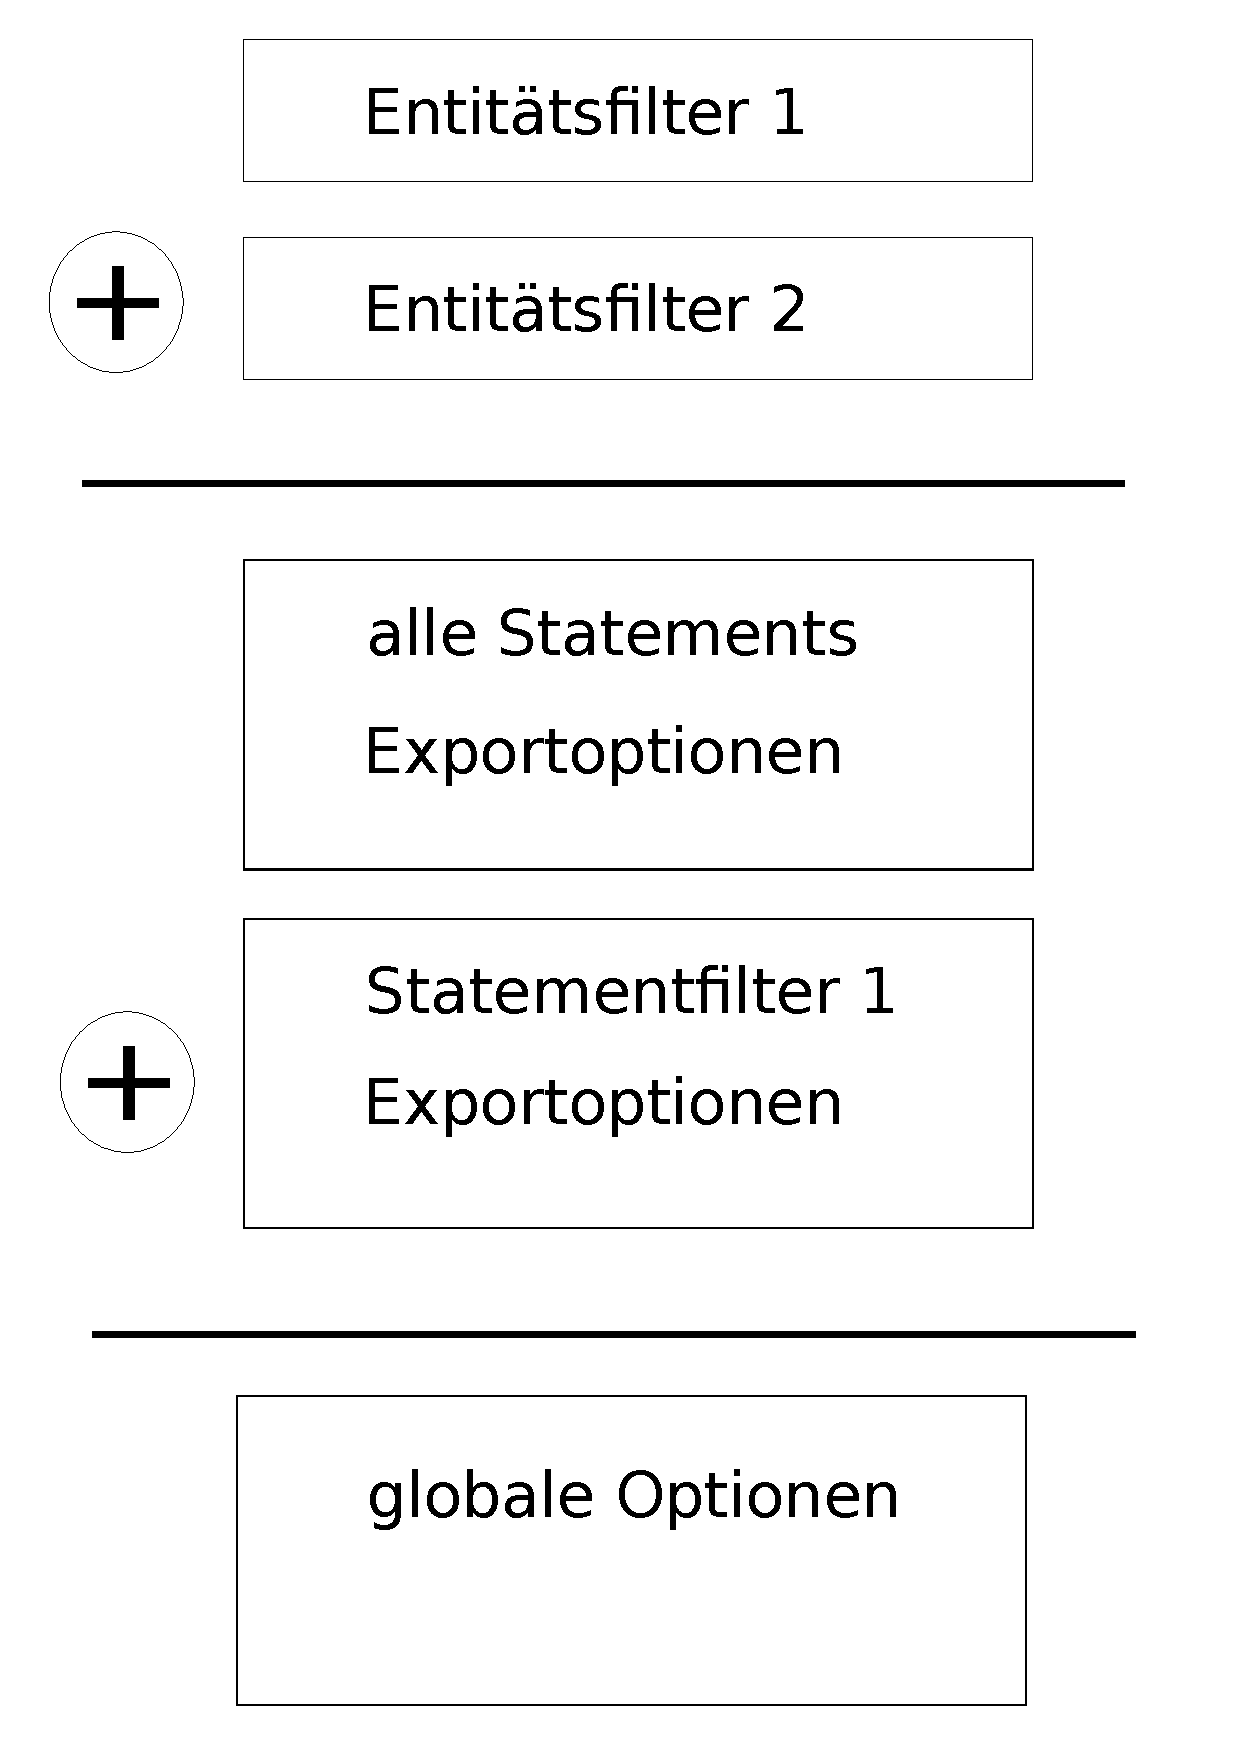
\includegraphics[width=\textwidth]{pics/ui-layout}
  \caption{Struktur des Interfaces zum Erstellen von Dumps}
  \label{fig:ui-layout}
\end{figure}

In Wikidata sind Statements immer ein Teil von Entities.
Folglich kann der Filterprozess konzeptionell in zwei Schritte zerlegt werden: zuerst werden die Entities ausgewählt, danach für diese Entities die zu exportierenden Statements.
Zusätzlich gibt es noch weitere globale Optionen, die sich nicht auf einzelne Statements beziehen, wie bspw. welche Sprachen exportiert werden sollen oder ob sitelinks von Entities exportiert werden sollen.
Diese Struktur des Interfaces ist in \cref{fig:ui-layout} dargestellt.

Für die Auswahl der Entitäten sind viele verschiedene Arten von Bedingungen denkbar.
Deswegen erlaubt das Interface die Kombination mehrerer Entitätsfilter von unterschiedlicher Art.
Für die erste Version der Software ist zunächst eine Filterart geplant, die Auswahlkriterien auf Basis von vorhandenen Statements unterstützt. 
Mit diesem Filter kann gefordert werden, dass Statements für bestimmte Prädikate bzw. bestimmte Prädikat/Objekt-Paare für eine Entität existieren.
Dieser Filter kann als Liste von Bedingungen im Interface dargestellt werden.
Weitere Filter sind denkbar, wie zum Beispiel alle Entitäten die Ergebnis einer SPARQL-Abfrage sind.
Prinzipiell könnte man Filter beliebig mit UND bzw. ODER kombinieren.
Mit dieser Freiheit würde das Interface allerdings sehr komplex.
Um das Interface einfach zu halten, werden Entitätsfilter deshalb immer mit ODER kombiniert, eine Entität wird demnach exportiert wenn mindestens einer der Filter zutrifft.
Es ist auch möglich, keinen Filter anzugeben.
In diesem Fall werden alle Entitäten exportiert (entsprechend den weiteren Regeln).

Für die Statements können Exportoptionen festgelegt werden.
Dafür gibt zum einen Standardoptionen, die für alle Statements der selektierten Entitäten angewendet werden.
Zusätzlich können für bestimmte Prädikate spezielle Exportoptionen festgelegt werden.
Damit können beispielsweise Qualifier nur bei bestimmten Prädikaten exportiert werden.
Die Optionen für den Export von Statements orientieren sich an der Struktur von Wikidata-Statements.
Für jede Komponente eines Statements (simple Statement, full Statement, Qualifier und Referenzen) kann einzeln festgelegt werden, ob diese generiert werden soll oder nicht.
Eine weitere Kategorie von Optionen betrifft den Export von Werten.
Dafür sind Schalter für den Export von einfachen Werten, komplexen Werten, normalisiert oder nicht normalisiert möglich.
Da das Backend das aber noch nicht unterstützt sind diese Optionen im Interface noch nicht vorhanden.
Insgesamt ist dieser Teil aber einfach erweiterbar, da die Optionen alle binär und somit einfach umsetzbar sind.

Die globalen Optionen sind auch größtenteils binär.
Hier kann eingestellt werden, ob Labels, Beschreibungen, Aliase bzw. sitelinks für selektierte Entitäten exportiert werden sollen.
Zudem findet sich hier die Option für die zu exportierenden Sprachen.
Man kann entweder keine Filterung der Sprachen vornehmen (alle Sprachen exportieren) oder eine Liste von Sprachen angeben.

An allen Stellen wo dies sinnvoll ist, bietet das Interface automatische Vervollständigung an.
Das trifft auf alle Eingabefelder für Entitäten zu, wobei Entitäten hier über ihr Label vervollständigt werden.
Außerdem wird eine Vervollständigung bei der Angabe von Sprachen angeboten, wobei eine feste Liste der möglichen Sprachen verwendet wird.

\section{Integration in existierende Infrastruktur}
Um die Anwendung zu betreiben, werden Ressourcen in Form von Rechenzeit für die Generierung der Dumps und Speicherplatz für die Archivierung benötigt.
Dazu lohnt es sich, bereits vorhandene Infrastruktur zu nutzen, um Aufwand und Kosten zu sparen.

Die Anwendung sollte auf Wikimedia-Servern betrieben werden, um die Verfügbarkeit auch in Zukunft unabhängig zu gewährleisten.
Für das Verarbeiten der Dumps und Betreiben des Web-Interfaces bietet sich hier die Wikimedia Toolforge\footnote{\url{https://tools.wmflabs.org/}} an.
Die Toolforge hat eine Grid-Engine, die zum Ausführung von längeren Jobs wie das Verarbeiten der Dumps geeignet ist, eine MySQL-Datenbank und einen Dienst zum Betreiben von Web-Services.
Die Alternative zur Toolforge wäre ein Wikimedia Cloud VPS Projekt\footnote{\url{https://wikitech.wikimedia.org/wiki/Portal:Cloud_VPS}}.
Es wird jedoch empfohlen, Cloud VPS nur zu verwenden, falls die Toolforge nicht ausreichend ist.
Deswegen wird für die Anwendung die Toolforge verwendet, da die Dienste in diesem Fall ausreichend sind.

Für die Archivierung der Dumps ist eine Integration mit Zenodo\footnote{\url{https://zenodo.org/}} vorgesehen.
Zenodo ist ein Datenarchivierungsdienst speziell für wissenschaftliche Zwecke und besitzt auch die Möglichkeit, einen Digital Object Identifier (DOI) zu registrieren, womit die Referenzierung von generierten Datensätzen leicht möglich ist.
Damit wird die Anforderung an Langzeitarchivierung erfüllt. 

Die Integration mit Zenodo funktioniert so, dass abgeschlossene Dumps als Datensatz zu Zenodo hochgeladen werden.
Dabei stellt sich die Frage, welcher Account für den Upload verwendet wird.
Zenodo bietet auch einen OAuth-Schnittstelle an, sodass es möglich wäre, die Dumps direkt zu einem Account des Nutzers hochzuladen.
Das erfordert es allerdings, dass Nutzer bereits einen Zenodo-Account besitzen.
Da die Implementierung von OAuth zudem zusätzliche Komplexität verursacht, verwendet die erste Version der Anwendung einen eigenen Account, der speziell dafür erstellt wurde.
Damit ist es mit einem Klick möglich, einen Dump zu Zenodo hochzuladen und den Dump dann über die DOI zu referenzieren, ohne das die Nutzer selbst einen Account bei Zenodo benötigen.        
\chapter{Implementierung}
\label{chap:implementation}

Die Anwendung besteht aus zwei Teilen: Backend und Frontend. Über das Frontend können Nutzer Aufträge für Dumps erstellen und existierende Dumps verwalten, während das Backend nur für die Generierung von Dumps zuständig ist.
Das Backend stellt dazu in regelmäßigen Abständen Anfragen an eine Datenbank, um nach neuen Aufträgen zu schauen welche vom Frontend hinzugefügt wurden.
In diesen Kapitel wird erst das Datenmodell vorgestellt, welches zur Kommunikation verwendet wird.
Danach wird die Implementierung von jeweils Frontend und Backend genauer beschrieben.

\section{Datenmodell}
\begin{figure}
  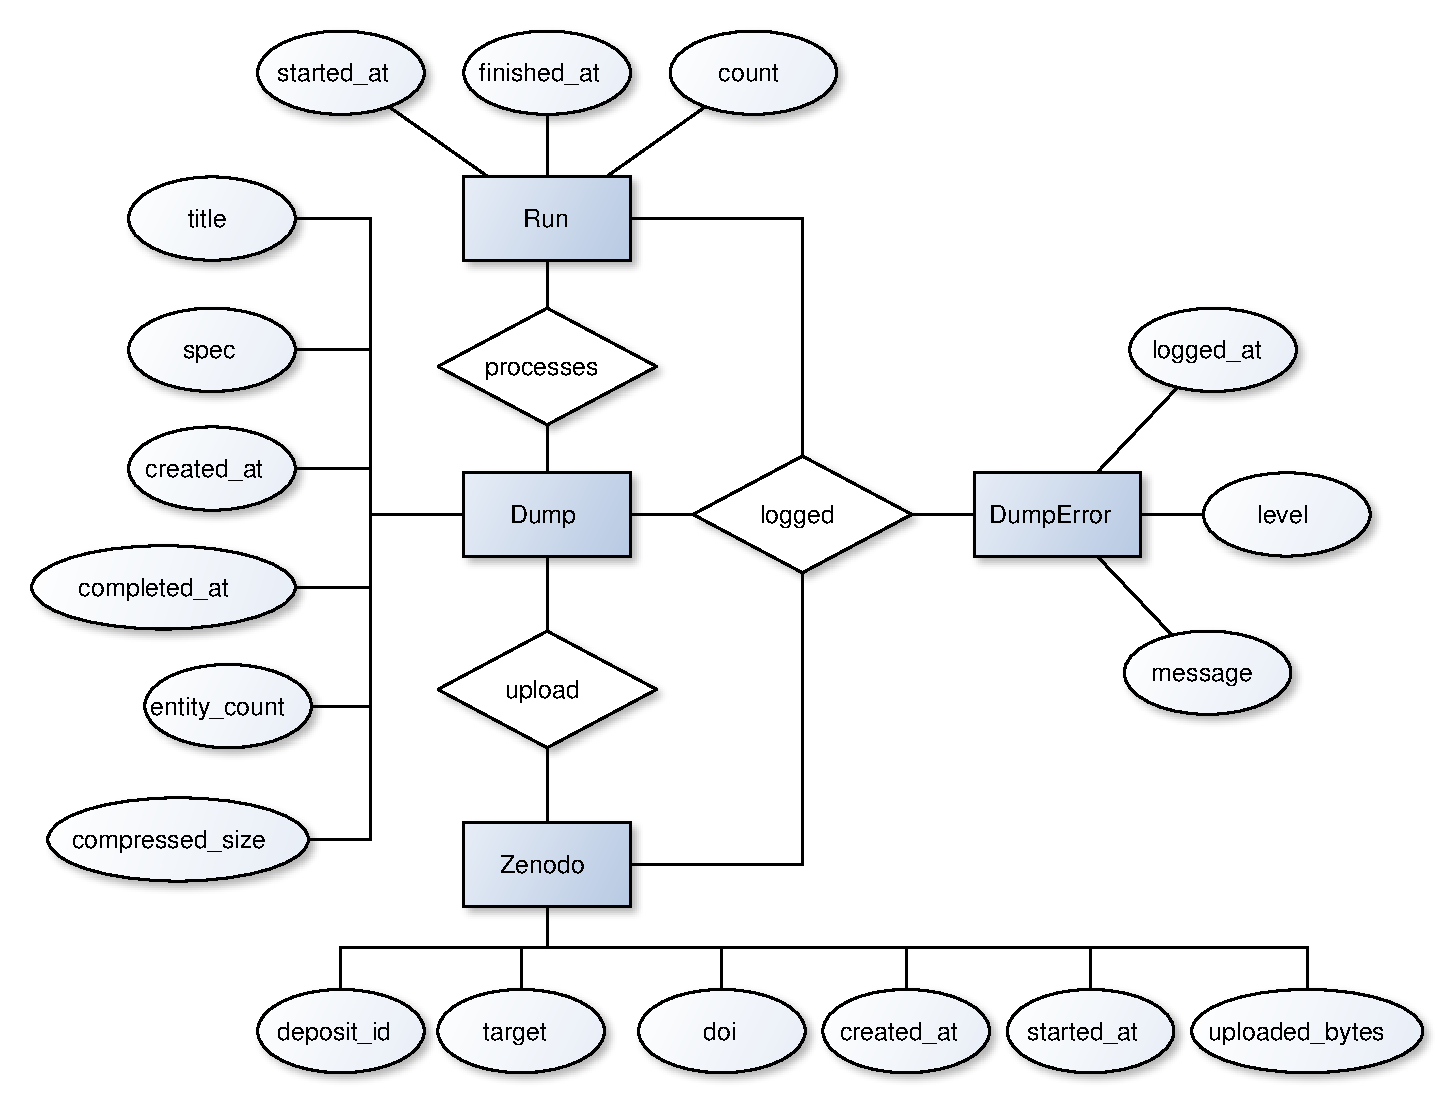
\includegraphics[width=\textwidth]{pics/db-er}
  \caption{Datenbankschema}
  \label{fig:db-er}
\end{figure}
Als zentraler Kommunikationspunkt zwischen Frontend und Backend wird eine Datenbank verwendet.
Man könnte dafür auch eine spezielle Message-Queue verwenden.
Die Datenbank wäre in diesem Fall allerdings trotzdem notwendig, um Metadaten zu den Aufträgen persistent zu speichern.
Um die Komplexität gering zu halten wurde deshalb auf eine separate Message-Queue verzichtet.

Eine Übersicht des Datenmodells liefert \cref{fig:db-er}.
Das zentrale Element ist der Dump, welcher alle Metadaten zu einem Auftrag speichert.
Neben ein paar einfachen Daten wie Titel (\verb|title|) und Zeitpunkt der Erstellung des Auftrags (\verb|created_at|) bzw. Fertigstellung (\verb|finished_at|) ist jeder Dump durch eine JSON-Spezifikation (\verb|spec|) charakterisiert. Zusätzlich hat der Dump auch Felder für Statistiken, wie die Anzahl der Entitäten (\verb|entity_count|) und Dateigröße (\verb|compressed_size|).

Für jeden Durchlauf des Backends wird ein \verb|Run| angelegt.
Die von diesem Durchlauf verarbeiteten Aufträge verweisen dann auf den \verb|Run|.
Damit der aktuelle Fortschritt ermittelt werden kann, wird die Anzahl der bereits verarbeiteten Entitäten in dem Attribut \verb|count| gespeichert.
Da die Anzahl von Entitäten in dem vollem Wikidata-Dump bekannt ist, lässt sich daraus der Fortschritt errechnen.

\section{Backend}
Für die Implementierung des Backends wird das Wikidata-Toolkit verwendet.
Da Wikidata-Toolkit in Java geschrieben ist, muss deswegen auch eine Java-kompatible Programmiersprache verwendet werden.
An dieser Stelle wurde Java gewählt, um auch die Wartbarkeit der Anwendung in Zukunft sicherzustellen, da Java im Vergleich zu anderen Programmiersprachen mit Java-Kompatibilität (wie zum Beispiel Scala\footnote{https://www.scala-lang.org/} oder Kotlin\footnote{\url{https://kotlinlang.org/}}) deutlich weiter verbreitet und bekannter ist.

Die Hauptschleife des Backends besteht aus zwei Phasen, Warten und Verarbeitung.
Während der wartenden Phase wird kontinuierlich auf neue Aufträge gewartet.
Sobald neue Aufträge verfügbar sind, wird die Verarbeitung gestartet. 
Neue Aufträge werden dann erst wieder nach Beendigung des aktuellen Verarbeitungsprozesses abgerufen.

Am Start befindet sich das Backend in der wartenden Phase.
Um neue Aufträge abzurufen, werden dazu periodische die in \cref{lst:backend-waiting} dargestellten SQL-Befehle in einer Transaktion ausgeführt.
Da in Zeile 6 nur Aufträge zugewiesen werden, die noch keinem \verb|Run| zugwiesen sind, kann diese Abfrage theoretisch auch von mehreren Prozessen gleichzeitg ausgeführt werden ohne dabei Kollisionen zu erzeugen.
Es ist so unmöglich, dass ein Auftrag mehr als einem \verb|Run| zugwiesen wird, was die Robustheit des Systems erhöht.
Falls diese Befehle keine Ergebnisse liefern (wenn keine neuen Aufträge vorliegen), wird eine definierte Zeit gewartet bevor dieser Vorgang wiederholt wird.
Diese Wartezeit führt gleichzeitig dazu, dass mehrere Aufträge gesammelt werden können, da die Verarbeitung nicht direkt beginnt.

\begin{lstlisting}[language=SQL, caption={Abrufen neuer Aufträge}, label={lst:backend-waiting}]
-- neuen Run erstellen
INSERT INTO run () VALUES ()
-- generated id: 1

-- Aufträge dem Run zuweisen
UPDATE dump SET run_id = 1 WHERE run_id IS NULL

-- Zugewiesene Aufträge abrufen
SELECT id, spec FROM dump WHERE run_id = :run
\end{lstlisting}

Zum Verarbeiten der Aufträge wurde der in Wikidata-Toolkit bereits vorhandene RDF-Export angepasst.
Der RDF-Export ist dabei als eine Klasse implementiert, welche das von Wikidata-Toolkit erwartete Interface \verb|EntityDocumentProcessor| implementiert (\cref{lst:wd-processor-interface}).

\begin{lstlisting}[language=Java, caption={EntityDocumentProcessor Interface}, label={lst:wd-processor-interface}]
  public interface EntityDocumentProcessor {
    void processItemDocument(ItemDocument itemDocument);
    void processPropertyDocument(PropertyDocument propertyDocument);
    void processLexemeDocument(LexemeDocument lexemeDocument);
  }
\end{lstlisting}


\cref{lst:export-pseudo} zeigt den Ablauf des Exports in Pseudocode.
Für jede Entität (Items, Properties und Lexemes) wird dazu zunächst überprüft, ob sie exportiert werden soll.
Nur wenn das der Fall ist, werden danach für jedes Statement die Optionen zum Export entsprechend der Filter-Spezifikation bestimmt. 
Wenn die Optionen feststehen, kann dann das Statement exportiert werden.
Aktuell werden Lexemes noch nicht untersützt, da Wikidata-Toolkit den RDF-Export dafür noch nicht implementiert hat.
Wenn ein Lexeme exportiert werden soll wird deshalb ein Fehler erzeugt.
Zusätzlich zu den Statements wird noch RDF für Labels, Descriptions, Aliases, Sitelinks und Metadaten zu der Entität erzeugt, falls entsprechend der Filter-Spezifikation verlangt.

\begin{lstlisting}[keywords={for,each,if,let}, caption={Export Pseudocode}, label={lst:export-pseudo}]
for each entity:
  if spec includes entity:
    if entity is lexeme: raise error
  
    if spec.labels: export entity labels
    if spec.aliases: export entity aliases
    if spec.descriptions: export entity descriptions

    for each statement:
      let options = get options for statement from spec
      export statement with options

    if spec.sitelinks: export entity sitelinks
    if spec.meta: export entity metadata
\end{lstlisting}

Wikidata-Toolkit unterstützt mehrere \verb|EntityDocumentProcessor|s gleichzeitig.
Damit können mehrere Aufträge in einem Durchlauf verarbeitet werden. 
Diese Funktionalität wird auch verwendet, um den aktuellen Fortschritt des Durchlaufs in der Datenbank zu aktualisieren.
Dazu zählt ein \verb|EntityDocumentProcessor| die Anzahl der verarbeiteten Entities mit und speichert diese regelmäßig in der \verb|run|-Tabelle der Datenbank.

\TODO{Auf StatementOptions / Spec interface eingehen}

\section{Frontend}
Das Frontend besteht aus einem Web-Interface zum Erstellen von Dump-Aufträgen und Verwaltung der existierenden Dumps.
Für dessen Implementierung wird hauptsächlich HTML/CSS mit Typescript verwendet, für die Auslieferung und Kommunikation mit der Datenbank gibt es aber auch eine kleine serverseitige Anwendung, welche in Python mit Flask geschrieben ist.

Der serverseitige Teil bietet dazu Endpunkte für das Erstellen, Suchen, Herunterladen und Abfrage von Informationen von Dumps an. Dazu werden vier Endpunkte bereitgestellt:
\begin{itemize}
\item \verb|POST /create| erstellt einen neuen Dump-Auftrag. Der Request-Body werden die Filter-Spezifikation sowie ein paar Metadaten (Titel, etc.) übergeben.
\item \verb|GET /dump/<id>| liefert eine Statusseite mit Informationen zu einem bestimmten Dump.
\item \verb|GET /dumps| gibt eine Liste aller Dumps zurück.
\item \verb|GET /download/<id>| lädt einen Dump herunter.
\end{itemize}


\chapter{Evaluation}
\label{chap:evaluation}    
\chapter{Fazit}
\label{chap:conclusion}
    

% --------------------------
% Back matter
% --------------------------

{%
\setstretch{1.1}
\renewcommand{\bibfont}{\normalfont\small}
\setlength{\biblabelsep}{0pt}
\setlength{\bibitemsep}{0.5\baselineskip plus 0.5\baselineskip}
\printbibliography[nottype=online]
\newrefcontext[labelprefix={@}]
\printbibliography[heading=subbibliography,title={Webpages},type=online]
}
\cleardoublepage

\newpage
\mbox{}

% **************************************************
% End of Document CONTENT
% **************************************************
\end{document}
